\subsubsection{Aplicaciones del Detector de Marcadores}

El detector de marcadores de referencia se emplea en tres contextos operativos distintos dentro del sistema, demostrando la versatilidad y robustez del algoritmo desarrollado.

\textbf{Aplicación 1: Corrección de Posición Horizontal}

En el contexto de corrección horizontal, el robot se posiciona frente a una cinta vertical y captura una imagen. El detector identifica la cinta y calcula la desviación horizontal del centroide respecto al centro de la imagen. Esta desviación, convertida a milímetros mediante calibración, se emplea para generar comandos de movimiento correctivo en el eje X que alinean el robot precisamente con la cinta.

Este procedimiento se ejecuta típicamente cuando el robot se aproxima a una estación de cultivo desde un lado, garantizando que el brazo de cosecha se encuentre correctamente alineado en dirección horizontal antes de descender.

\textbf{Aplicación 2: Corrección de Posición Vertical}

En el contexto de corrección vertical, el robot se posiciona sobre una cinta horizontal y captura una imagen. El detector identifica la cinta y calcula la desviación vertical del centroide respecto al centro de la imagen. Esta desviación se emplea para generar comandos de movimiento correctivo en el eje Y que alinean verticalmente el robot con la cinta.

Este procedimiento se ejecuta cuando el robot ha alcanzado aproximadamente la altura de una estación de cultivo, refinando su posición vertical antes de intentar la cosecha. La precisión de esta corrección es crítica dado que las lechugas presentan geometrías verticales variadas y el punto de corte debe ubicarse con precisión de ±2 mm.

\textbf{Aplicación 3: Escaneo Horizontal para Mapeo}

Durante la fase de mapeo autónomo del entorno, el robot recorre horizontalmente el espacio de trabajo detectando cintas verticales que marcan las posiciones de las estaciones de cultivo. En este contexto, el detector opera en modo continuo: mientras el robot se desplaza en dirección X, captura imágenes periódicamente y ejecuta el algoritmo de detección.

Cuando se detecta una cinta vertical, el sistema registra la coordenada X actual como una posición válida de estación. Para evitar detecciones duplicadas de la misma cinta debido a la continuidad del movimiento, se implementa un mecanismo de debouncing temporal: tras detectar una cinta, se inhabilita la detección durante 2 segundos, tiempo suficiente para que el robot se aleje de la cinta y avance hacia la siguiente.

Este escaneo horizontal permite construir automáticamente un vector de coordenadas X que identifica todas las columnas de estaciones sin conocimiento a priori de la geometría del sistema. Esta capacidad de auto-descubrimiento hace que el sistema sea adaptable a configuraciones variables del invernadero.

\begin{figure}[H]
\centering
\begin{subfigure}[b]{0.48\textwidth}
    \centering
    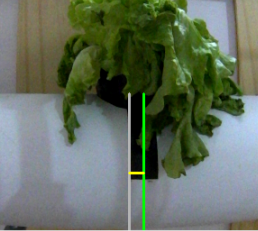
\includegraphics[width=\textwidth]{imagenes/detector_marcadores_5_lineas_verticales.png}
    \caption{Detección de cinta vertical para corrección horizontal}
\end{subfigure}
\hfill
\begin{subfigure}[b]{0.48\textwidth}
    \centering
    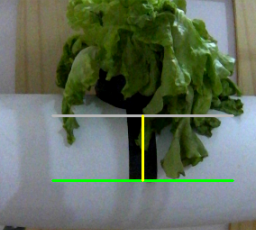
\includegraphics[width=\textwidth]{imagenes/detector_marcadores_5_lineas_horizontales.png}
    \caption{Detección de cinta horizontal para corrección vertical}
\end{subfigure}
\caption{Aplicaciones del detector de marcadores en ambos ejes de corrección}
\label{fig:aplicaciones_marcadores}
\end{figure}

\subsubsection{Particularidades de Implementación por Aplicación}

Aunque el algoritmo central es idéntico en las tres aplicaciones, existen diferencias en parámetros y configuración adaptados a cada contexto:

\textbf{Modo de Corrección (horizontal y vertical):}
\begin{itemize}
\item El robot está estático durante la captura y análisis
\item Se emplea el sistema de scoring completo para máxima precisión
\item Se ejecuta calibración espacial para conversión píxel-milímetro
\item Se implementa corrección iterativa hasta convergencia (tolerancia < 1 mm)
\item Tiempo típico por corrección: 1-2 segundos
\end{itemize}

\textbf{Modo de Escaneo Horizontal:}
\begin{itemize}
\item El robot está en movimiento lento (20 mm/s) durante las capturas
\item Se simplifica el scoring, priorizando velocidad sobre precisión máxima
\item No se requiere conversión a milímetros, solo detección binaria presencia/ausencia
\item Se implementa debouncing temporal en lugar de espacial
\item Tiempo típico por detección: 50-80 ms
\end{itemize}

Esta adaptabilidad demuestra que un algoritmo robusto basado en principios sólidos puede servir múltiples propósitos con ajustes mínimos de configuración, reduciendo la complejidad del sistema global.
